\documentclass[a4paper,12pt]{report}

\usepackage[T1]{fontenc}
\usepackage[utf8]{inputenc}
\usepackage[english]{babel}

\usepackage[hidelinks]{hyperref}
\usepackage{graphicx}
\usepackage{caption}

\title{Connector - Reference manual }
\author{Gianluigi Forte}

\usepackage{listings}
\usepackage{color}

\lstdefinelanguage{asymptote}{%
keywords=[1]{import, unitsize, add, shift,
 show, arc, include}, %pour asymptote + geometry
keywords=[2]{label, draw, dot, geometry, grid, triangleabc, perpendicularmark},% pour les autres extensions
keywords=[3]{pair, triangle, path}, % pour les classes
keywords=[4]{lightgray, black, gray, red}, %pour les couleurs
keywords=[5]{bp, pt, cm,  % unités
 N, E, S, W, NE, SE, SW, NW,
 NNE, ENE, ESE, SSE, SSW, WSW, WNW, NNW},% points cardinaux
comment=[l]{//},
otherkeywords={ -- , .. , :: , \^\^},
sensitive=true,
%morecomment=[s]{/*}{*/},
%string=[d]",
moredelim=*[s][\color{black}]{"}{"},
moredelim=**[s][\color{black}]{{$}{$}}
}


\lstset{%
language=asymptote,
keywordstyle=[1]\ttfamily\bfseries\color{black},
keywordstyle=[2]\ttfamily\color{black},
keywordstyle=[3]\ttfamily\bfseries,
keywordstyle=[4]\ttfamily\color{black},
keywordstyle=[5]\ttfamily\bfseries\color{black},
identifierstyle=\ttfamily\color{black},
firstnumber=5
}% à compléter au besoin
%
%

\begin{document}
\maketitle

\section*{Introduction}

Connector is a library written in \emph{Asymptote} language to generate figures of electronic schematics.
\LaTeX and \emph{Asymptote}, differently from other programs like Word or Write, are languages designed
to produce documents with the best quality outputs for prints or presentations starting from a description,
of the content to be produced, expressed programmatically in a source code text file and then produced in
output after the compilation process. The idea behind the \emph{connector} library is to provide a ready
to use set of functions written in Asymptote language to draw electrical components, link them with connection
(wires), decorate with labels and produce the output figure as pdf or png files to be embedded in a larger
Latex document or any kind of other usage like websites, videos, presentations and so on. 
An example of the image generated with \emph{connector} is shown in figure \ref{threePhaseInverterExample}.
The source code \texttt{ThreePhaseInverter.asy} to produce the figure is included in the library.

\begin{figure}[ht]
  \centering
  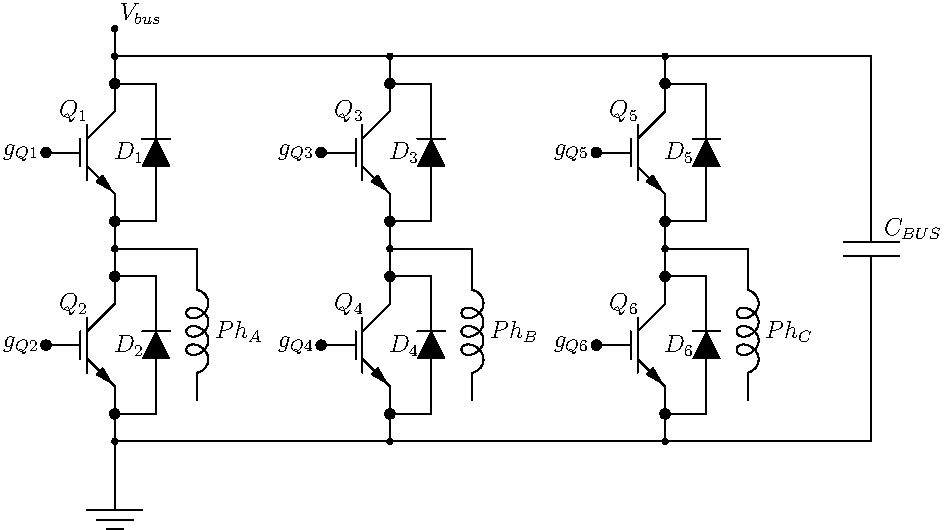
\includegraphics[width=1.0\textwidth]{ThreePhaseInverter.pdf}
  \caption{Example of schematics generated with \emph{connector}}
  \label{threePhaseInverterExample}
\end{figure}

\section*{Electronic Symbols}

The following list of components have been included in the libary and can be used out-of-the-box.
\begin{itemize}
\item node
\item resistor
\item capacitor
\item inductor
\item fuse
\item diode
\item relay
\item relay SPDT
\item IGBT
\item MOS
\item power ground
\item signal ground
\end{itemize}

In the folowing figures are shown the components, the anchor points with index number, and the origin position $(0,0)$ indicated with a red cross.

In figure \ref{nodeInfo} is shown a generic node symbol. See \texttt{nodeInfo.asy} code to reproduce the figure.

\begin{figure}[ht]
\centering
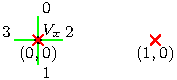
\includegraphics[width=0.2\textwidth]{nodeInfo}
\caption{Example of use of a generic node}
\label{nodeInfo}
\end{figure}

In figure \ref{resistorInfo} is shown a resistor symbol. See \texttt{resistorInfo.asy} code to reproduce the figure.

\begin{figure}[ht]
\centering
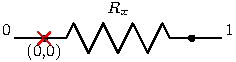
\includegraphics[width=0.5\textwidth]{resistorInfo}
\caption{Example of use of resistor}
\label{resistorInfo}
\end{figure}

In figure \ref{capaciorInfo} is shown a capacitor symbol. See \texttt{capaciorInfo.asy} code to reproduce the figure.

\begin{figure}[ht]
\centering
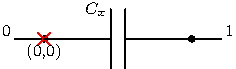
\includegraphics[width=0.5\textwidth]{capacitorInfo}
\caption{Example of use of capacitor}
\label{capaciorInfo}
\end{figure}

In figure \ref{inductorInfo} is shown an inductor symbol. See \texttt{inductorInfo.asy} code to reproduce the figure.

\begin{figure}[ht]
\centering
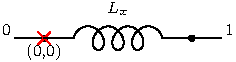
\includegraphics[width=0.5\textwidth]{inductorInfo}
\caption{Example of use of inductor}
\label{inductorInfo}
\end{figure}

In figure \ref{fuseInfo} is shown a fuse symbol. See \texttt{fuseInfo.asy} code to reproduce the figure.

\begin{figure}[ht]
\centering
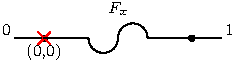
\includegraphics[width=0.5\textwidth]{fuseInfo}
\caption{Example of use of fuse}
\label{fuseInfo}
\end{figure}

In figure \ref{diodeInfo} is shown a diode symbol. See \texttt{diodeInfo.asy} code to reproduce the figure.

\begin{figure}[ht]
\centering
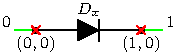
\includegraphics[width=0.5\textwidth]{diodeInfo}
\caption{Example of use of diode}
\label{diodeInfo}
\end{figure}

In figure \ref{relayInfo} is shown a relay symbol. See \texttt{relayInfo.asy} code to reproduce the figure.

\begin{figure}[ht]
\centering
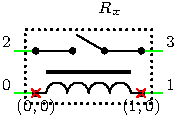
\includegraphics[width=0.45\textwidth]{relayInfo}
\caption{Example of use of relay}
\label{relayInfo}
\end{figure}

In figure \ref{relaySPDTInfo} is shown a relay SPDT symbol. See \texttt{relaySPDTInfo.asy} code to reproduce the figure.

\begin{figure}[ht]
\centering
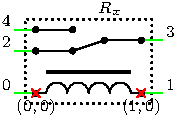
\includegraphics[width=0.45\textwidth]{relaySPDTInfo}
\caption{Example of use of relay SPDT}
\label{relaySPDTInfo}
\end{figure}

In figure \ref{igbtInfo} is shown an IGBT symbol. See \texttt{igbtInfo.asy} code to reproduce the figure.

\begin{figure}[ht]
\centering
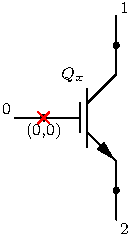
\includegraphics[width=0.3\textwidth]{igbtInfo}
\caption{Example of use of igbt}
\label{igbtInfo}
\end{figure}

In figure \ref{mosInfo} is shown a MOS transistor symbol. See \texttt{mosInfo.asy} code to reproduce the figure.

\begin{figure}[ht]
\centering
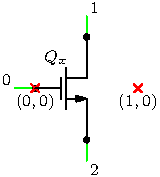
\includegraphics[width=0.3\textwidth]{mosInfo}
\caption{Example of use of MOS}
\label{mosInfo}
\end{figure}

In figure \ref{gndPowerInfo} is shown a power ground symbol. See \texttt{gndPowerInfo.asy} code to reproduce the figure.

\begin{figure}[ht]
\centering
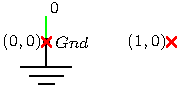
\includegraphics[width=0.2\textwidth]{gndPowerInfo}
\caption{Example of use of power ground symbol}
\label{gndPowerInfo}
\end{figure}

In figure \ref{gndSignalInfo} is shown a signal ground symbol. See \texttt{gndSignalInfo.asy} code to reproduce the figure.

\begin{figure}[ht]
\centering
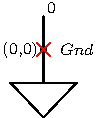
\includegraphics[width=0.2\textwidth]{gndSignalInfo}
\caption{Example of use of signal ground symbol}
\label{gndSignalInfo}
\end{figure}

\section*{Connectors}

It is possible to draw connectors (wires) between symbols with the function \texttt{drawAnchorConnector}. In particular the
connection is done starting from one anchor point to another ancor point that are defined in the sybmol (see from figure \ref{nodeInfo} to figure \ref{gndSignalInfo}).
The path of the connector is automatically computed by the library in the best way and is drown according the direction
of the ancor point. The figure \ref{connectorExample} show an example of connections
between generic objects.

\begin{figure}[ht]
  \centering
  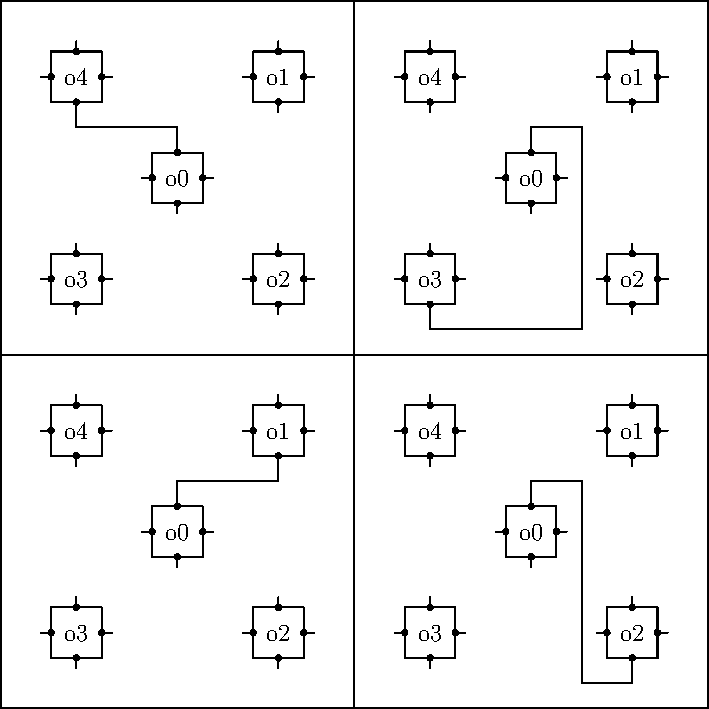
\includegraphics[width=1.0\textwidth]{N-S}
  \caption{Example of use of connectors between objects}
  \label{connectorExample}
\end{figure}

The \texttt{drawAnchorConnector} function takes as parameters respectively: the first object to be connected,
the anchor point index of the first object, the second object to be connected and the index of the anchor point
of the second object.

\texttt{drawAnchorConnector(obj1, Anchor1, obj2, Anchor2)}

There are also other three optional parameters that can be used to set the aspect of the connection ($r_1,r_2,r_3$).


\end{document}